%! Author = gra
%! Date = 23.03.24

% Preamble
\begin{flushleft}
    \subsubsection{Benchmarking - Vorgehen}
    \paragraph{YugabyteDB}
    Zuerst muss die Datenbank erstellt und die Tablespaces erzeugt werden, die genauen Schritte sind im \hyperref[subsubsec:yugabytedb_benchmarking_sql]{Anhang - YugabyteDB Benchmark SQL} zu finden.\\    Anschliessend
    Anschliessend muss pro Lauf erst initialisiert werden, dann kann mit dem eigentlichen Benchmarking gestartet werden.\\
    Alle Benchmarking-Commands sind im \hyperref[subsec:yugabytedb_benchmarking_commands]{Anhang - YugabyteDB Benchmarking Commands} zu finden.
    \paragraph{Patroni}
    Als die 250GiB DB getestet wurde, zeigte sich, dass die Parameter nicht darauf optimiert waren.\\
    Die Standby-Server konnten die \texttt{WAL}-Files nicht mehr abarbeiten, so stauten sich auf dem Primary die Files und die Disk lief jeweils voll.\\
    Es wurden demnach folgende Parameter angepasst:
    \begin{description}
        \item \textbf{max\_connections}\hfill \\Damit die 7000 Transaktionen sicher abgesetzt werden können.
        \item \textbf{superuser\_reserved\_connections}\hfill \\Mindestens 10 \texttt{postgres}-Verbindungen müssen gemacht werden können.
        \item \textbf{max\_worker\_processes}\hfill \\Damit genügend Worker vorhanden sind, um die \texttt{WAL}-Files abzuarbeiten, wurde deren Zahl auf 16 erhöht.
        \item \textbf{wal\_log\_hints}\hfill \\Stellt sicher, dass der gesamte Diskpage-inhalt ins \texttt{WAL} geschrieben wird.
        \item \textbf{max\_wal\_senders}\hfill \\Um den Replikations-Throughput zu erhöhen, wurden 16 Sender aktiviert
        \item \textbf{max\_replication\_slots}\hfill \\Damit die 16 Sender auch auf der Gegenseite abgearbeitet werden,\\müssen die entsprechenden Slots bereitgestellt werden.
        \item \textbf{wal\_keep\_size}\hfill \\Damit die \texttt{WAL}-Files nicht zu gross werden und somit auch das Replication-Lag,\\wurde die Grösse auf 1GiB reduziert.\\Das zwingt den Primary dazu, die \texttt{WAL}-Files nur bis zu Maximal 1GiB aufzubewahren bevor sie archiviert werden.\\Das ist wichtig, wenn Diskspace nicht im Überfluss vorhanden ist.
        \item \textbf{wal\_level}\hfill \\Der Level wurde auf logical gesetzt, damit alle Informationen geschrieben werden.
        \item \textbf{wal\_buffers}\hfill \\Der Buffer wurde auf 16MiB erhöht.
        \item \textbf{wal\_writer\_delay}\hfill \\Wenn der WAL-Writer einen Flush durchgeführt hat, geht er in ein Timeout.\\Dies wurde auf 20ms heruntergesetzt, damit rasch wieder geschrieben wird.
        \item \textbf{wal\_writer\_flush\_after}\hfill \\Definiert, ab welcher Grösse der Cache des WAL-Writters auf die Disk geschrieben wird.\\Wurde auf 1MiB gesetzt um rasch auf die Disk schreiben zu können.
        \item \textbf{min\_wal\_size}\hfill \\Damit die \texttt{WAL}-Files nicht zu schnell repliziert werden und die Standby-Server aber auch der Primary-Server nicht überlastet werden,\\sollen die Files mindestens 1GiB gross werden bevor sie repliziert werden.
        \item \textbf{max\_wal\_size}\hfill \\Auf der anderen Seite soll trotzdem nicht zu lange gewartet werden,\\die maximale grösse wurde auf 5GiB begrenzt.
        \item \textbf{commit\_delay}\hfill \\Maximal 20ms soll gewartet werden, bevor ein Transaktions-Commit geflushed wird.
        \item \textbf{commit\_siblings}\hfill \\Maximal 10 Transktionen sollen offen bleiben, bevor es zu einem Flush kommt.
        \item \textbf{checkpoint\_timeout}\hfill \\Die maximale Zeit zwischen den Checkpoints soll 5min betragen.
        \item \textbf{archive\_mode}\hfill \\Um Diskspace zu sparen sollen die \texttt{WAL}-Files nicht aktiviert werden.
        \item \textbf{checkpoint\_completion\_target}\hfill \\Ab 95\% des Checkout-Timeouts soll mit dem Abschluss begonnen werden.
        \item \textbf{max\_standby\_archive\_delay}\hfill \\Erst nach zehn Minuten sollen die Standby-Queries abgebrochen werden.\\Ist notwendig, da es wegen der grossen Datenmenge und entsprechendem lag sonst schnell zum Abbruch kommen kann.
        \item \textbf{max\_standby\_streaming\_delay}\hfill \\Beim normalen Standby soll die Zeit nur 3min sein.
        \item \textbf{wal\_receiver\_status\_interval}\hfill \\Alle 60 sekunden soll der Status ausgetauscht werden.
        \item \textbf{max\_logical\_replication\_workers}\hfill \\Acht logische Replication worker sollen zum einsatz kommen.
        \item \textbf{max\_sync\_workers\_per\_subscription}\hfill \\Es soll die maximale Anzahl an workern (8) für das parallelisieren verwendet werden.
        \item \textbf{shared\_buffers}\hfill \\Der gesamte Server hat 16GiB Memory, \(\frac{1}{4}\) davon soll als Buffer dienen, also 4GiB.
        \item \textbf{maintenance\_work\_mem}\hfill \\1GiB soll zur Verfügung stehen für den \Gls{AUTOVACUUM}-Job oder Maintenance-Jobs wie das indexieren usw.
        \item \textbf{work\_mem}\hfill \\Der ganze \Gls{PostgreSQL Cluster} soll 12GiB Memory zur Verfügung haben.
        \item \textbf{temp\_file\_limit}\hfill \\Damit für das erzeugen von Primary Keys, Foreign-Keys oder Indizes genügend Platz vorhanden ist,\\sollen temporäre Tabellen 200GiB Diskspace allokieren können.
        \item \textbf{vacuum\_cost\_delay}\hfill \\Der \Gls{AUTOVACUUM}-Job soll maximal 2ms ruhen.
        \item \textbf{vacuum\_cost\_limit}\hfill \\Der gesamte Prozess darf maximal zehn sekunden Schlafen.
        \item \textbf{bgwriter\_delay}\hfill \\Der Hintergrundprozess soll nur 10ms ruhen.
        \item \textbf{bgwriter\_lru\_maxpages}\hfill \\Maximal dürfen 800 Buffers vom Hintergrundprozess beschrieben werden.
        \item \textbf{bgwriter\_lru\_multiplier}\hfill \\Insgesamt sollen beim nächsten Schreibzyklus 5 x soviel neue Writer erzeugt werden, wie im aktuellen Zyklus benötigt werden.
    \end{description}
    Mit diesen Parametern konnte die Datenmenge verarbeitet werden.
\end{flushleft}
\begin{flushleft}

    \paragraph{StackGres - Citus}
    Beim Benchmarking zeigten sich die Grenzen des Citus Shardings.\\
    Bereits beim Lesen der Anleitung fiel auf, dass für das Sharding der Tabellen \texttt{pgbench\_accounts} und \texttt{pgbench\_history} jeweils neu initialisiert wurde\cite{6CJFR7RM}.\\
    Das hat einen besonderen Grund.\\
    Wenn die Tabellen mittels des SELECT-Statements \texttt{create\_distributed\_table} die Tabellen einem Sharding unterzogen werden sollen, kommt es zu einer Fehlermeldung.\\
    Die Shards würden mit folgenden SQL-Statements erzeugt:
\lstset{style=gra_codestyle}
\begin{lstlisting}[language=sql, caption=Citus - Benchmarking - Distributed Table Sharding,captionpos=b,label={lst:benchmarking_distributed_table_sharding},breaklines=true]
SELECT create_distributed_table('pgbench_branches', 'bid');
SELECT create_distributed_table('pgbench_tellers', 'tid');
SELECT create_distributed_table('pgbench_accounts', 'aid');
SELECT create_distributed_table('pgbench_history', 'aid');
\end{lstlisting}
    Ursache ist, dass eine Distributed Table offenbar keine Foreign Key Constraints erlaubt.\\
    \texttt{pgbench} erzeugt aber gleich mehrere davon:\\
    \begin{figure}[H]
        \centering
        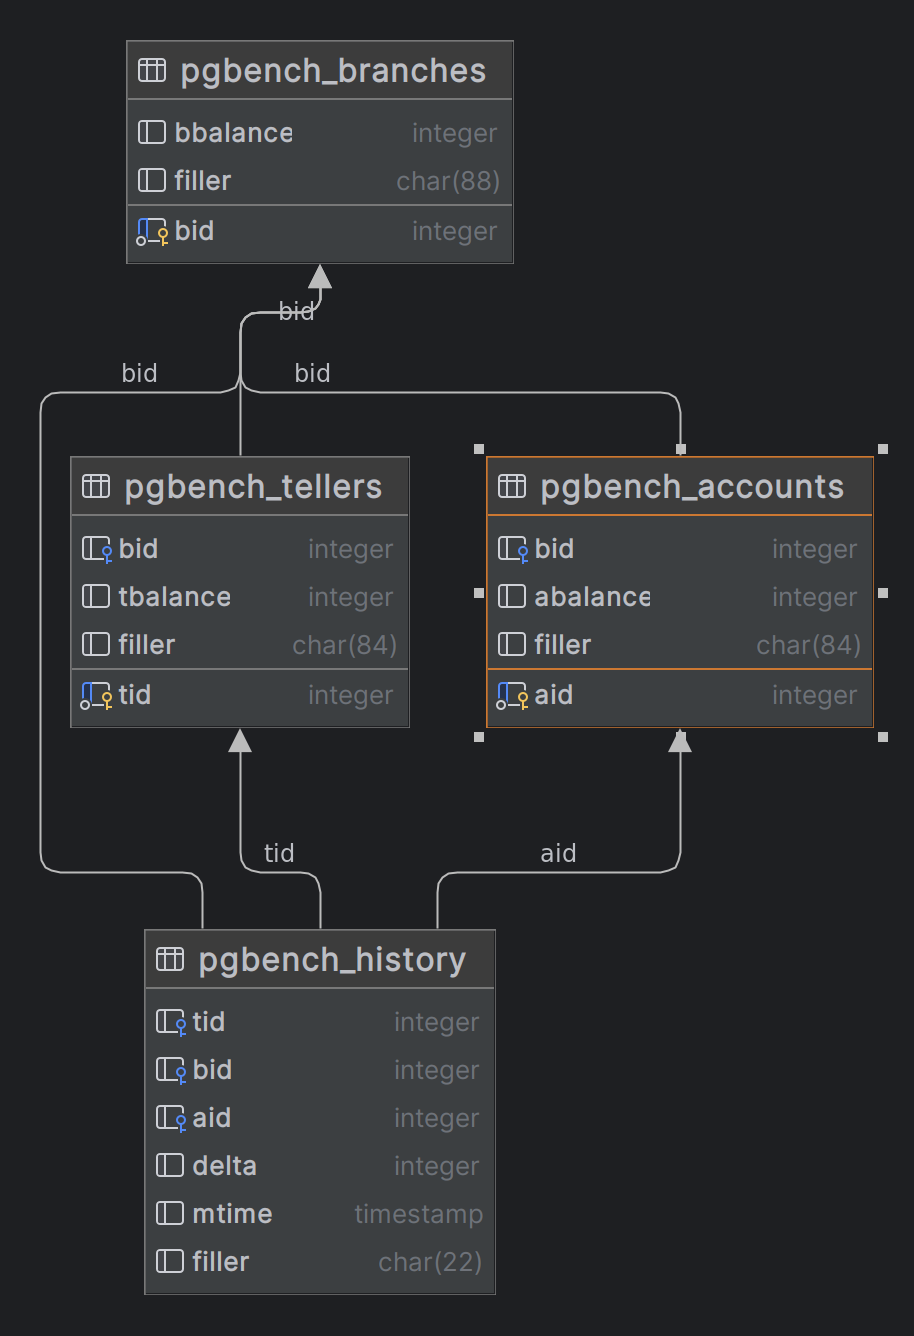
\includegraphics[width=0.5\linewidth]{source/implementation/evaluation/benchmarking/stackgres_citus/pgbench_accounts}
        \caption{Benchmarking - ERD pgbench}
        \label{fig:pgbench_accounts}
    \end{figure}
    Ein Schema-Based Sharding ist nicht möglich, da \texttt{pgbench} nur die DB als Parameter übernimmt.\\
    Die Tabellen werden zudem immer dropped bevor sie neu erzeugt und gefüllt werden, das Sharding kann daher nur im Nachgang gemacht werden.\\
\end{flushleft}
\begin{flushleft}
    Die Lösung für das Benchmarking bestand also darin, sogenannte Reference Tables zu erstellen:
\lstset{style=gra_codestyle}
\begin{lstlisting}[language=sql, caption=Citus - Benchmarking - Reference Table Sharding,captionpos=b,label={lst:benchmarking_reference_table_sharding},breaklines=true]
SELECT create_reference_table('pgbench_branches');
SELECT create_reference_table('pgbench_tellers');
SELECT create_reference_table('pgbench_accounts');
SELECT create_reference_table('pgbench_history');
\end{lstlisting}
    Referenzierte Tabellen werden auf alle Shards repliziert und erfüllen somit die Anforderung an das Sharding.\\
    Diese Art des Sharding wäre allerdings nur für kleinere Tabellen, Multi-Tenant Sharding (wenn Tabellen bei allen Tenants verfügbar sein sollen),\\
    Tabellen die mit verschiedenen Distributed Tables gejoint werden oder wenn eben, wie in unserem Fall, Foreign-Key Constraints im Spiel sind\cite{KPPLMKD4}.
\end{flushleft}
\begin{flushleft}
    Aber auch in diesem Fall muss das Sharding im Nachgang des \texttt{pgbench}-Inits gemacht werden.\\
    Bei den kleinen Tabellen geht das relativ flot, doch gerade bei der Tabelle \texttt{pgbench\_accounts} dauert es sehr lange.\\
    Lang genug, dass eine eigene betrachtung beim Benchmarking angezeigt wurde.\\
    Leider zeigte sich auch bei den mixed-Benchmarks, anders als bei den dql-Benchmarks, dass diese Art des Sharding nicht sehr performant ist.
\end{flushleft}
\begin{flushleft}
    Wie bei Patroni und YugabyteDB auch, musste für den letzten Benchmark die StorageClass auf die neue Disk verlegt werden.\\
    Aber anders als bei YugabyteDB reichten 250GiB nicht mehr, wie bei Patroni lag die Ursache beim Generieren der Primary- und Foreign-Keys.
\end{flushleft}
\begin{flushleft}
    Es zeigte sich aber auch rasch, dass der Coordinator die gleiche Grösse annahm, wie die Shard-Pods.\\
    Das führte dazu, dass beim letzten Benchmark nur noch 2 Shard-Instanzen deployt werden konnten,\\
    da sonst bei jeder Disk nochmals mindestens 350GiB hinzugefügt hätte werden müssen (da sich der Coordinator den Node mit einem Shard geteilt hätte und der Coordinator auf jedem Node erscheinen könnte).\\
    Es hätten also für die Evaluation 3 x 700GiB (plus noch 3 x 50GiB für den Rest), also 3 x 750GiB, allokiert werden müssen.\\
    Auf diesen Mehraufwand wurde verzichtet um das \Gls{SAN} und somit das Daily Business nicht zu stark zu belasten.
\end{flushleft}
\begin{flushleft}
    Alle Benchmarking-Commands und SQLs zur ermittlung der grösse sind im \hyperref[subsec:stackgres_citus_benchmarking_commands]{Anhang - StackGres - Citus Benchmarking Commands} zu finden.
    \subsubsection{Benchmarks}
    Der vergleich zwischen den verschiedenen Varianten.\\
\end{flushleft}
\begin{flushleft}

\end{flushleft}
\begin{flushleft}
    Bei den Transaktionen pro Sekunden gilt, je höher der Wert, umso besser das Ergebnis.\\
%    Zuerst die Ergebnisse mit den mixed-Transaktionen:
%    \begin{figure}[H]
%        \centering
%        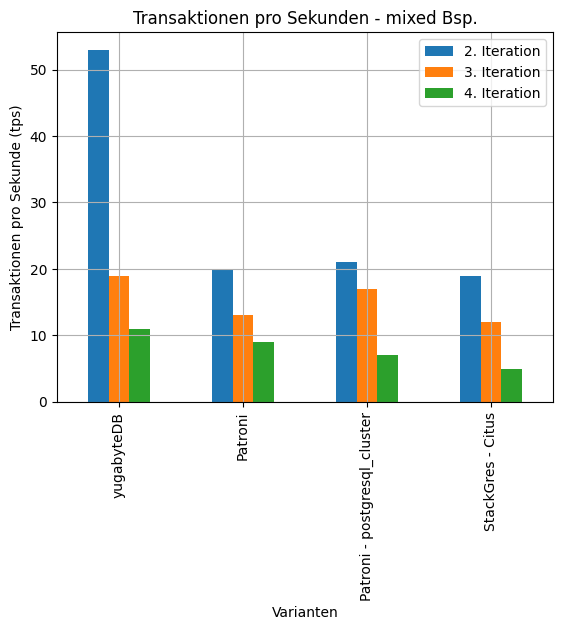
\includegraphics[width=0.5\linewidth]{source/pandas_data_chart_plotter/tps_mixed}
%        \caption{Benchmarks - tps mixed}
%        \label{fig:tps_mixed}
%    \end{figure}
%
%    Folgend die reinen Select-Transaktionen.
%    \begin{figure}[H]
%        \centering
%        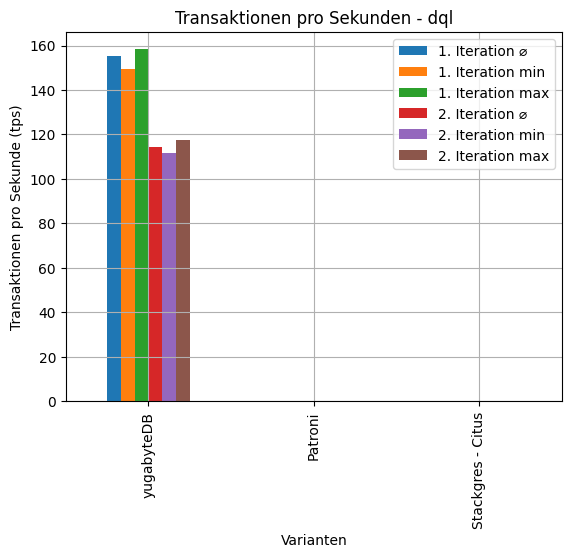
\includegraphics[width=0.5\linewidth]{source/pandas_data_chart_plotter/tps_dql}
%        \caption{Benchmarks - tps dql}
%        \label{fig:tps_dql}
%    \end{figure}

    \begin{figure}[H]
        \centering
        \subfloat{{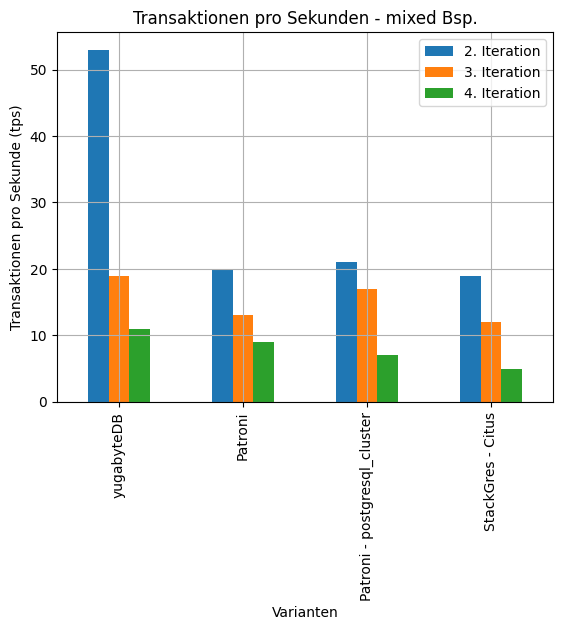
\includegraphics[width=0.47\linewidth]{source/pandas_data_chart_plotter/tps_mixed} }}%
        \qquad
        \subfloat{{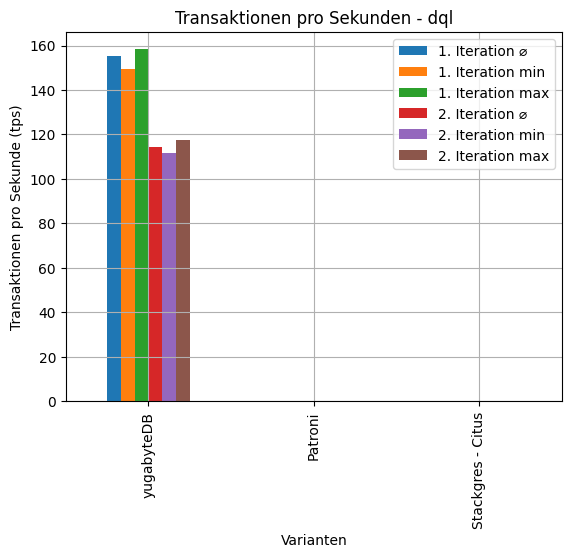
\includegraphics[width=0.47\linewidth]{source/pandas_data_chart_plotter/tps_dql} }}%
        \caption{Benchmarks - tps}
        \label{fig:tps_varianten}
    \end{figure}
    Bei der Latenz ist es genau andersrum, je höher der Wert desto schlechter schnitt die Variante ab.\\
%    Auch hier zuerst wieder die mixed-Transaktionen:
%    \begin{figure}[H]
%        \centering
%        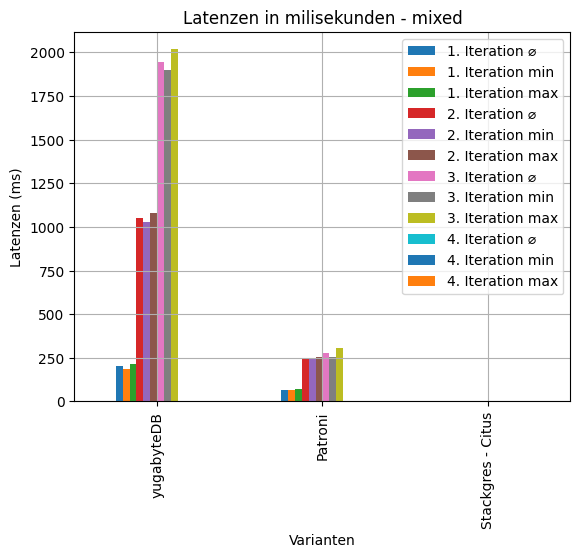
\includegraphics[width=0.5\linewidth]{source/pandas_data_chart_plotter/latency_mixed}
%        \caption{Benchmarks - latency mixed}
%        \label{fig:latency_mixed}
%    \end{figure}
%
%    Folgend die Select-Transaktionen:
%    \begin{figure}[H]
%        \centering
%        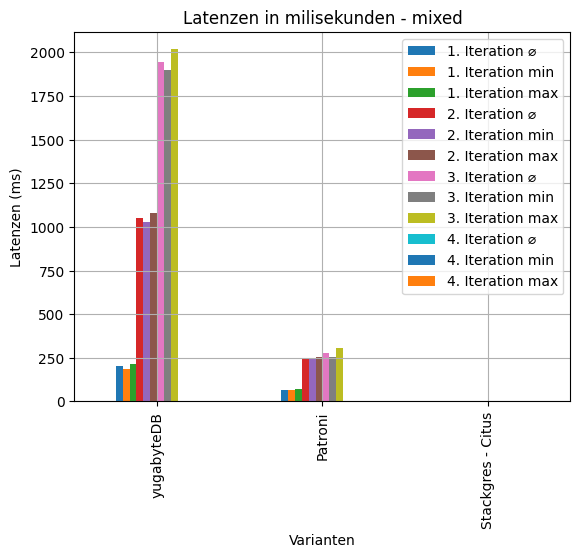
\includegraphics[width=0.5\linewidth]{source/pandas_data_chart_plotter/latency_dql}
%        \caption{Benchmarks - latency dql}
%        \label{fig:latency_dql}
%    \end{figure}

    \begin{figure}[H]
        \centering
        \subfloat{{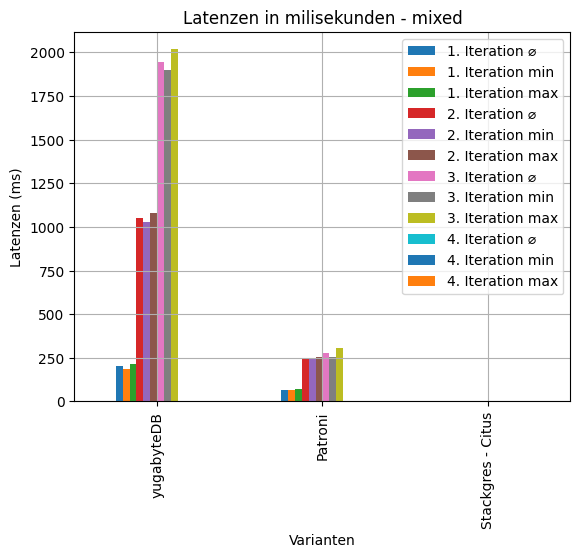
\includegraphics[width=0.47\linewidth]{source/pandas_data_chart_plotter/latency_mixed} }}%
        \qquad
        \subfloat{{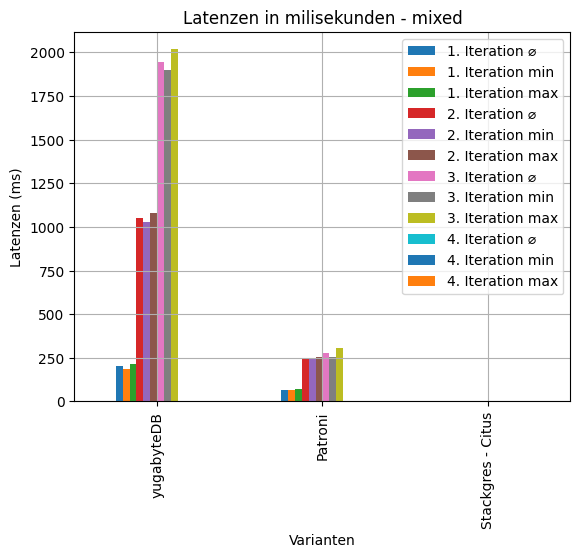
\includegraphics[width=0.47\linewidth]{source/pandas_data_chart_plotter/latency_dql} }}%
        \caption{Benchmarks - latency}
        \label{fig:latency_varianten}
    \end{figure}
\end{flushleft}
\begin{flushleft}
    Die ersten beiden läufe mit Patroni wurde erst nur mit der Asynchronen Standard-Replikation von Patroni vorgenommen.\\
    Später wurden die Benchmarks mit der Synchronen Replikation wiederholt.\\
    Daraus ergab sich die Möglichkeit, beide Methoden direkt zu vergleichen:
    \begin{figure}[H]
        \centering
        \subfloat{{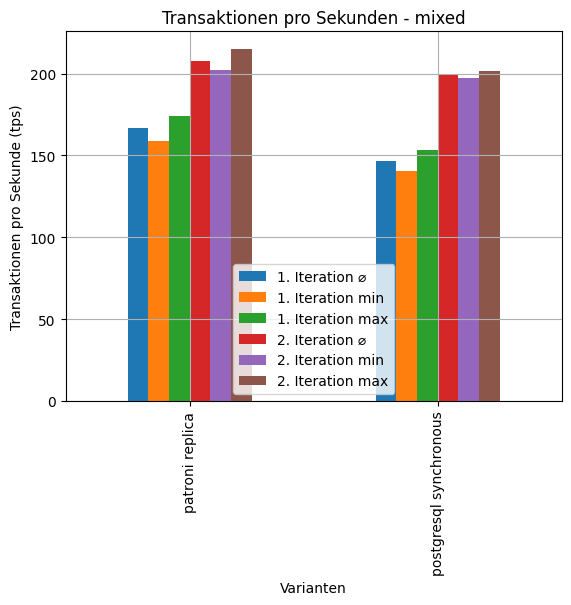
\includegraphics[width=0.47\linewidth]{source/pandas_data_chart_plotter/tps_patroni_replica_mixed} }}%
        \qquad
        \subfloat{{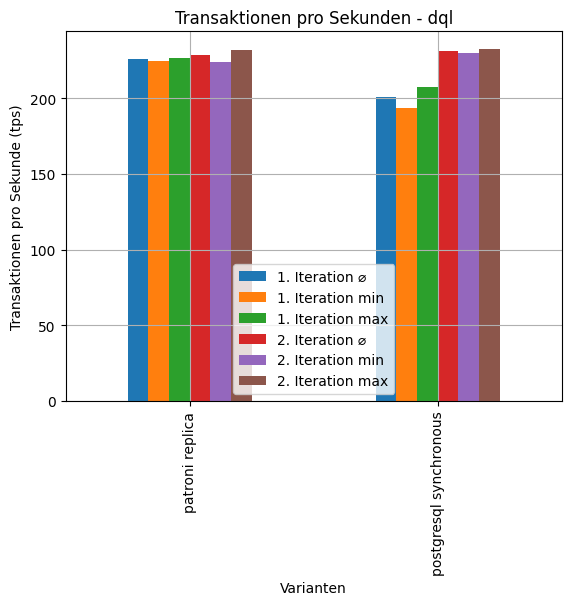
\includegraphics[width=0.47\linewidth]{source/pandas_data_chart_plotter/tps_patroni_replica_dql} }}%
        \caption{Benchmarks - tps Patroni Replica}
        \label{fig:tps_patroni_replica}
    \end{figure}
    \begin{figure}[H]
        \centering
        \subfloat{{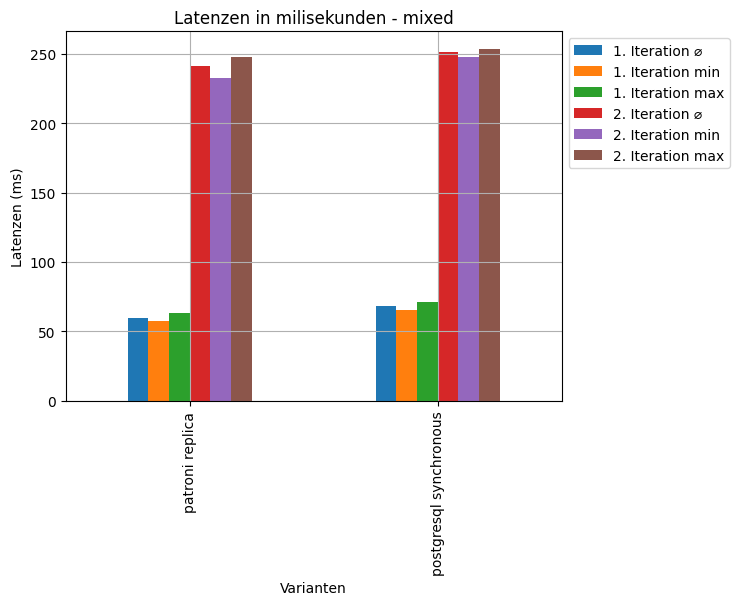
\includegraphics[width=0.47\linewidth]{source/pandas_data_chart_plotter/latency_patroni_replica_mixed} }}%
        \qquad
        \subfloat{{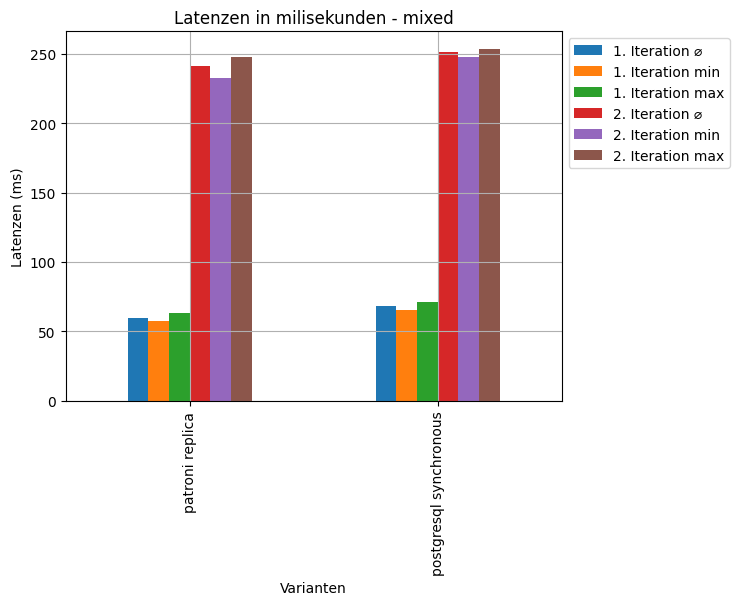
\includegraphics[width=0.47\linewidth]{source/pandas_data_chart_plotter/latency_patroni_replica_dql} }}%
        \caption{Benchmarks - latency Patroni Replica}
        \label{fig:latency_patroni_replica}
    \end{figure}
    Die Asynchrone Replikation ist dabei ein klein wenig schneller als die Synchrone Replikation.
\end{flushleft}
\begin{flushleft}
    Ein weiterer Benchmark sind die Fehler, die bei den DML-Transktionen beim mixed-Benchnmark auftreten können.
    \begin{figure}[H]
        \centering
        \subfloat{{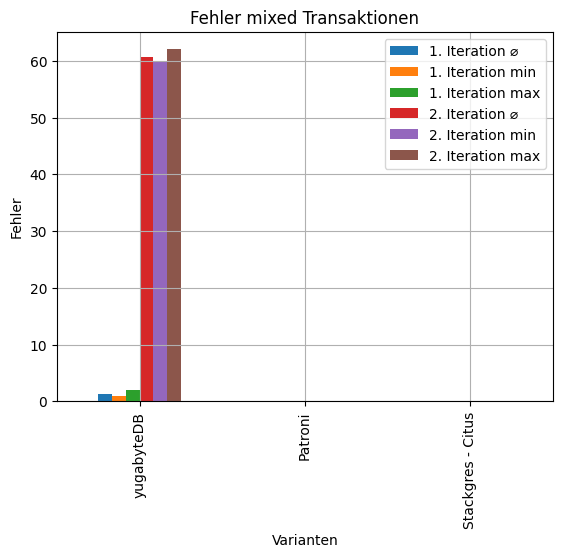
\includegraphics[width=0.47\linewidth]{source/pandas_data_chart_plotter/pgbench_errors_absolute} }}%
        \qquad
        \subfloat{{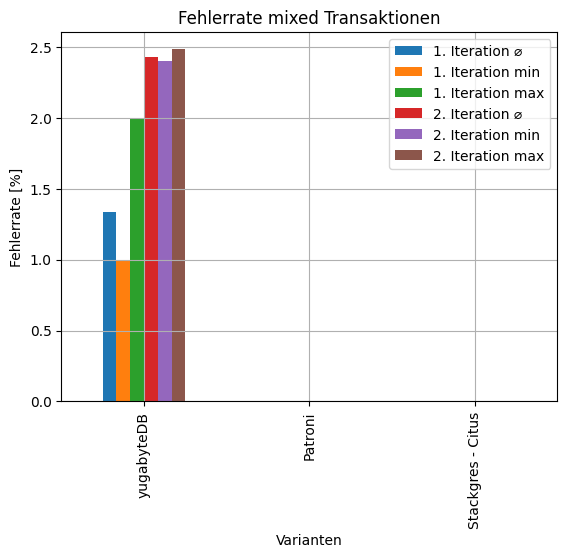
\includegraphics[width=0.47\linewidth]{source/pandas_data_chart_plotter/pgbench_errors_percentage} }}%
        \caption{Benchmarks - Fehler bei mixed-Transaktionen}
        \label{fig:pgbench_errors}
    \end{figure}
\end{flushleft}
\begin{flushleft}
    Ebenfalls ein wichtiger Benchmark ist die Zeit, die benötigt wird, um mittels \texttt{pgbench} initialisiert die Tabellen zu erstellen.
    \begin{figure}[H]
        \centering
        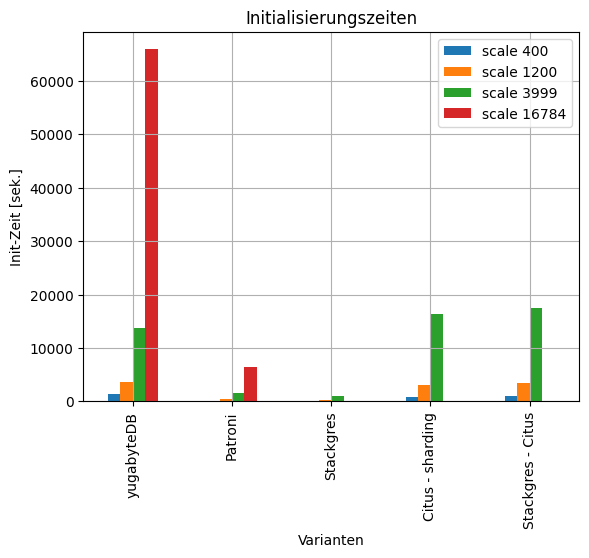
\includegraphics[width=0.5\linewidth]{source/pandas_data_chart_plotter/initializing_time_sec}
        \caption{Benchmarks - Initialisierungszeit - sekunden}
        \label{fig:initializing_time_sec}
    \end{figure}
    \begin{figure}[H]
        \centering
        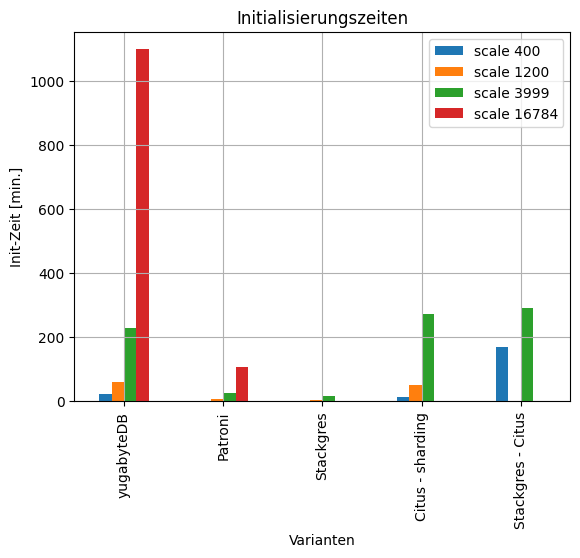
\includegraphics[width=0.5\linewidth]{source/pandas_data_chart_plotter/initializing_time_min}
        \caption{Benchmarks - Initialisierungszeit - minuten}
        \label{fig:initializing_time_min}
    \end{figure}
    \begin{figure}[H]
        \centering
        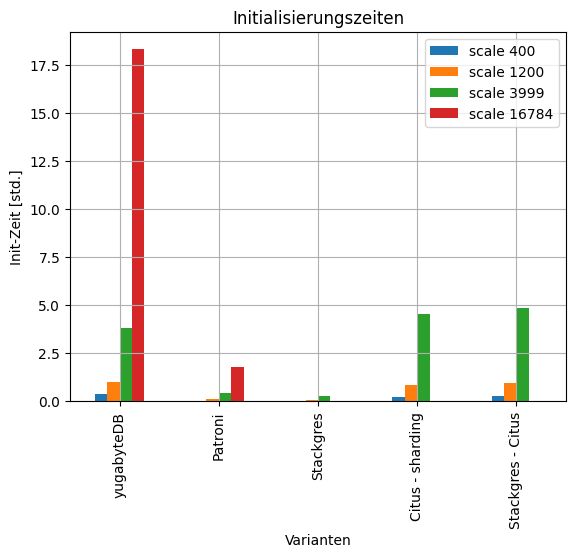
\includegraphics[width=0.5\linewidth]{source/pandas_data_chart_plotter/initializing_time_hour}
        \caption{Benchmarks - Initialisierungszeit - stunden}
        \label{fig:initializing_time_hour}
    \end{figure}
    Dabei fällt auf, mit Patroni werden die Tabellen am schnellsten geladen.\\
    StackGres selber generiert ebenfalls wesentlich schneller als YugabyteDB.\\
    Werden dann aber die Tabellen in Shards aufgeteilt, verändert sich die Initialisierungszeit zuungunsten von StackGres - Citus.


\end{flushleft}
